\documentclass[11pt,a4paper]{article}

%======================================================================
% Title, author and date
%======================================================================

\title{
	Projektdokumentation\\
	Transportüberwachungssystem Roadrunner
}
\author{
	Franziskus Domig, B.Sc.\\
		\and
	Stefan Gassner, B.Sc.\\
		\and
	Wolfgang Halbeisen, B.Sc.\\
		\and
	Matthias Schmid, B.Sc.\\	
}
\date{\today}

%======================================================================
% Packages
%======================================================================

%%%%%%%%%%%%%%%%%%%%%%%%%%%%%%%%%%%%%%%%%%%%%%%%%%%%%%%%%%%%%%%%%%%%%
% Packages

% für \hyphenation mit Umlauten
\usepackage[T1]{fontenc}
\usepackage[utf8]{inputenc}
\usepackage[ngerman,english]{babel}

% Times-Roman-Schrift (auch für mathematische Formeln)
\usepackage{mathptmx} 

% comments
\usepackage{verbatim} 

% Zum Setzen von URLs
\usepackage{color}
\usepackage{alltt}
\definecolor{darkred}{rgb}{.25,0,0}
\definecolor{darkgreen}{rgb}{0,.2,0}
\definecolor{darkmagenta}{rgb}{.2,0,.2}
\definecolor{darkcyan}{rgb}{0,.15,.15}

\usepackage[plainpages=false,bookmarks=true,bookmarksopen=true,colorlinks=true,
  linkcolor=darkred,citecolor=darkgreen,filecolor=darkmagenta,
  menucolor=darkred,urlcolor=darkcyan]{hyperref}

% Zeilenabstand
\renewcommand{\baselinestretch}{1.5}

% anhang
\usepackage[toc,page]{appendix}

% pdflatex: Bilder in den Formaten .jpeg, .png und .pdf
% latex: Bilder im .eps-Format
\usepackage{graphicx}

\usepackage{fancyhdr} % Positionierung der Seitenzahlen
\fancyhead{}
\fancyfoot[C]{\Roman{page}}
\renewcommand{\headrulewidth}{0pt}
\setlength{\headheight}{13.6pt} % behebt headheight Warning

 % behebt headheight Warning
\setlength{\headheight}{13.6pt}

% Korrektes Format für Nummerierung von Abbildungen (figure) und
% Tabellen (table): <Kapitelnummer>.<Abbildungsnummer>
\makeatletter
\@addtoreset{figure}{section}
\renewcommand{\thefigure}{\thesection.\arabic{figure}}
\@addtoreset{table}{section}
\renewcommand{\thetable}{\thesection.\arabic{table}}
\makeatother

% Listings für Sourcecode
\usepackage{listings}
  \usepackage{courier}
 \lstset{
        basicstyle=\footnotesize\ttfamily, % Standardschrift
        numbers=left,               % Ort der Zeilennummern
        numberstyle=\tiny,          % Stil der Zeilennummern
        %stepnumber=2,               % Abstand zwischen den Zeilennummern
        numbersep=5pt,              % Abstand der Nummern zum Text
        tabsize=2,                  % Groesse von Tabs
        extendedchars=true,         %
        breaklines=true,            % Zeilen werden Umgebrochen
        keywordstyle=\color{red},
        frame=b,         
        keywordstyle=[1]{\color{DarkSkyBlue}},    % Stil der Keywords
        keywordstyle=[2]{\color{DarkScarletRed}},    %
        keywordstyle=[3]{\bfseries},    %
        keywordstyle=[4]{\color{DarkPlum}},    %
        keywordstyle=[5]{\color{SkyBlue}},    %
		stringstyle={\color{Chocolate}},
        showspaces=false,           % Leerzeichen anzeigen ?
        showtabs=false,             % Tabs anzeigen ?
        xleftmargin=17pt,
        framexleftmargin=17pt,
        framexrightmargin=5pt,
        framexbottommargin=4pt,
        backgroundcolor=\color{Aluminium1},
        showstringspaces=false,      % Leerzeichen in Strings anzeigen ?
		%language=php
		morekeywords=[1]{Interface,return,static,function}
}
    %\DeclareCaptionFont{blue}{\color{blue}} 

  %\captionsetup[lstlisting]{singlelinecheck=false, labelfont={blue}, textfont={blue}}
  \usepackage{caption}
\DeclareCaptionFont{white}{\color{white}}
\DeclareCaptionFormat{listing}{\colorbox[cmyk]{0.43, 0.35, 0.35,0.01}{\parbox{\textwidth}{\hspace{15pt}#1#2#3}}}
\captionsetup[lstlisting]{format=listing,labelfont=white,textfont=white, singlelinecheck=false, margin=0pt, font={bf,footnotesize}}
\renewcommand\lstlistingname{Codeblock}
 

\sloppy % Damit LaTeX nicht so viel über "overfull hbox" u.Ä. meckert

% Ränder
\addtolength{\topmargin}{-16mm}
\setlength{\oddsidemargin}{40mm}
\setlength{\evensidemargin}{40mm}
\addtolength{\oddsidemargin}{-1in}
\addtolength{\evensidemargin}{-1in}
\setlength{\textwidth}{13cm}
\addtolength{\textheight}{34mm}
%______________________________________________________________________

% Verhindert Hurenkinder & Schusterjungen
\clubpenalty = 10000
\widowpenalty = 10000
\displaywidowpenalty = 10000



%======================================================================
% PDF settings
%======================================================================

\hypersetup{
	pdfauthor = {
		Franziskus Domig, B.Sc;
		Stefan Gassner, B.Sc.;
		Wolfgang Halbeisen, BSc;
		Matthias Schmid, B.Sc.
	},
	pdftitle = {Projekt Dokumentation Roadrunner},
	pdfkeywords = {Roadrunner, Dokumentation, Transport, Logistik,
		Transportüberwachung},
}

%======================================================================
%      Document
%======================================================================

\begin{document}
	
\selectlanguage{ngerman}

\pagestyle{empty} % Vorerst keine Seitenzahlen
\pagenumbering{alpha} % Unsichtbare alphabetische Nummerierung

\begin{center}


\includegraphics[width=60mm]{files/logo-fhv.png}

\vspace{4cm}
{\large\textbf{Projektdokumentation}}\vspace{.5cm}

{\LARGE Transportüberwachungssystem Roadrunner}

\end{center}

\vspace{13cm}


\begin{tabular}{ll}
	Projektteam: & Franziskus Domig, BSc; Stefan Gassner, BSc;\\
	     	& Wolfgang Halbeisen, BSc; Matthias Schmid, BSc\\
	Bearbeitung: & Dornbirn, im Sommersemester 2011\\
	Betreuer:    & Prof.(FH) DI Wolfgang Auer\\
\end{tabular}

%______________________________________________________________________

\clearpage
\pagestyle{fancy}
\pagenumbering{roman} % Römische Seitenzahlen
\setcounter{page}{1}

\begin{abstract}
	In dieser Arbeit wird die Erstellung eines Transportüberwachungssystems
		für Arzneimittel erläutert. Es werden die Komponenten einer mobilen
		Applikation für die	Android Plattform beschrieben, ein Backendserver
		mit CouchDB erläutert sowie die Überwachung mit einer Webapplikation
		dargestellt. Um das	implementierte System für ein reales Szenario
		verwenden zu können, werden abschließend die wirtschaftlichen Aspekte
		analysiert.
\end{abstract}

% Abstract in english
\begin{otherlanguage}{english}
	\begin{abstract}
		This paper describes the development of a monitoring and tracing system
			for pharmaceutical products. Furthermore the development of a
			mobile application for the Android platform as well as the
			backendserver with a CouchDB database and the corresponding
			webapplication are described in detail. An economical reflection on
			the developed system is given in a concluding section.
	\end{abstract}
\end{otherlanguage}

\clearpage
\tableofcontents

\clearpage
\pagenumbering{arabic}
\setcounter{page}{1}

% Geändertes Format für Seitenränder, arabische Seitenzahlen
\fancyfoot[CO]{\thepage}

\section{Motivation}

In diesem Projekt haben wir uns auf die Entwicklung von Software konzentriert.
	Hardware sowie entsprechende Sensoren werden simuliert. Wir haben uns in
	neuen Technologien, teilweise sogar in Beta-Versionen, eingearbeitet und 
	diese exzessiv in diesem Projekt verwendet.

Als Softwareentwicklungsprozess wurde \emph{Test-Driven-Development} gewählt.
	Hierzu wurden nahezu alle entwickelten Komponenten mit \emph{Unit-Tests}
	getestet sowie wenn möglich auf einem \emph{Continius-Integration}-Server
	bei jeder Änderung automatisiert getestet.
	
TODO: mehr Inhalt

\clearpage
\section{Projektanforderungen}
\label{sec:requirements}

Das Ziel dieses Projekts ist es, ein System zur lückenlosen Transportüberwachung
	zu entwickeln. Hierzu sollen Produkt, welche erst im Rahmen des Projekts zu
	spezifizieren sind, überwacht werden. Es soll nach einem Transport möglich
	sein, eindeutig nachvollziehen zu können, welche Sensor-Daten zu jedem
	Zeitpunkt aufgezeichnet wurde.
	
TODO: mehr Inhalt

\clearpage
\section{Systembeschreibung und -architektur}
\label{sec:system}

In diesem Abschnitt werden die in diesem Projekt verwendeten Technologien
	erläutert. Insbesondere werden die Gründe beschrieben, weswegen diese
	Technologien eingesetzt und anderen vorgezogen werden. Die Vor- sowie
	Nachteile der entsprechenden Technologien werden gegenübergestellt und
	besprochen. Zugleich werden die entsprechenden Technologien auf ihre
	Tauglichkeit in einem real logistischen Szenario geprüft.

\subsection{Mobiles Gerät auf Basis von Android}

Bei diesem Transportüberwachungssystem sollten laut den in
	Kapitel~\ref{sec:requirements} spezifizierten Anforderungen eine lückenlose
	und ständige Überwachung sichergestellt werden. Somit müssen Sensorendaten
	laufend auf ein Backendsystem übertragen werden. Hierzu bietet sich
	die \emph{Android}\footnote{vgl. \url{http://www.android.com/}} Plattform
	als Grundlage für eine mobile Applikation an.
	
Mit Android als Grundlage können gleich mehrere Aspekte abgedeckt werden. Jedes
	Fahrzeug wird mit einem Android Smartphone ausgestattet und ist somit nicht
	nur telefonisch erreichbar sondern gleichzeitig kann die komplette
	Transportüberwachung damit erreicht werden.
	
Mit der entwickelten Applikation lassen sich Gegenstände einladen indem diese
	via Barcode in das System übernommen werden. Ab diesem Zeitpunkt wird dieser
	Gegenstand ständig überwacht und via CouchDB (siehe Abschnitt~\ref{subsec:couchdb})
	mit dem Backensystem synchronisiert. Auf der Webapplikation (siehe
	Abschnitt~\ref{subsec:webapplication}) können die Produkte bzw. die Lieferung,
	welche aus mehreren Produkten bestehen kann nun auf einer Karte	nachverfolgt
	werden sowie die jeweiligen Daten der Temperatursensoren (siehe
	Abschnitt~\ref{subsec:nodejs}) bis zum ausladen überprüft werden.
		
Auch in einem realen Szenario lässt sich Android hervorragend einsetzten. Es ist
	mittlerweile in Version~3.1 (15. Juni 2011) verfügbar und weit verbreitet.
	Die von Google bereitgestellten \emph{Google Apps for Business}\footnote{vgl.
	\url{http://www.google.com/apps/intl/de/business/index.html}} können die
	Smartphones per Fernwartung administriert werden. Dabei können auch
	Applikations-Updates an alle registrierten Smartphones verteilt werden.
	Somit ist auch eine einfache Lösung für das Deployment von neuen Versionen
	gegeben.
	
Im Kapitel~\ref{sec:android} wird die in diesem Projekt erstellte Android Applikation
	beschrieben.

\subsection{Verteiltes Datenbansystem CouchDB}
\label{subsec:couchdb}

Bei einem Transportüberwachungssystem ist die Datensicherung ein
	wichtiger Aspekt. In diesem Abschnitt wird die Datenverwaltung
	betrachtet und erläutert welches System für dieses
	verwendet wird.

In diesem Projekt wurde durch die in Kapitel~\ref{sec:requirements} spezifizierten
	Anforderungen ein Fokus auf die Verteiltheit des Systems gelegt. Es fallen
	durch die mobile Transportüberwachung Daten auf mobilen Geräten an, welche
	mit einem Backendsystem synchronisiert werden müssen. Aus diesem Grund wurde
	für das Datenbanksystem kein klassisches System in Betracht gezogen. Um einen
	neuen Ansatz in der Datenpersistierung zu erlernen, wurde das verteilte
	und dokumentbasierte Datenbankmanagementsystem \emph{CouchDB}\footnote{vgl.
	\url{http://couchdb.apache.org/}} verwendet.

In einem real logistischen Szenario muss auf die Skalierbarkeit sowie die
	Robustheit von CouchDB betrachtet werden. Klassische relationale
	Datenbankmanagementsysteme bringen durch die bereits sehr gut entwickelten
	Versionen vor allem einen Vorteil in der Robustheit und Stabilität. Dennoch,
	CouchDB wird bereits seit 2005 entwickelt und liegt aktuell in der stabilen
	Version 1.1.0 (6. Juni 2011) vor und wird bereits in mehreren kommerziellen
	Projekten wie beispielsweise in Ubuntu \cite{Murphy09}[S. 1] eingesetzt.

Einen detaillierten Überblick der Verwendung von CouchDB in diesem Projekt
	wird in Kapitel~\ref{sec:couchdb} gegeben.

\subsection{Webapplikation mit dem Framework Silex}
\label{subsec:webapplication}

Um ein benutzerfreundliches und einfaches Backendsystem
	für dieses Projekt zu erstellen, wurde auf mehrere bereits bestehende Frameworks
	zurückgegriffen. \emph{Silex}\footnote{vgl. \url{http://silex-project.org}} ist
	ein	Mikroframework für PHP 5.3. Es basiert wiederum auf dem Kern des
	\emph{Symfony2}\footnote{vgl. \url{http://symfony.com}} Frameworks.
	
Mit diesem Framework lassen sich einfache Webapplikationen sehr effizient in einer
	Model-View-Controller Umgebung implementieren. Durch die schöne Trennung der
	jeweiligen Schichten sowie der leichten Testbarkeit ist Silex für dieses
	Projekt hervorragend geeignet.
	
Für ein Szenario in der Realität kann Silex sehr gut eingesetzt werden solange das
	System einfach und klein ist. Mit mehr in dem Backendsystem implementierten
	Usecases sollte ein Wechsel zu Symfony2 in Betracht gezogen werden, da sich
	damit deutlich komplexere Anwendungsfälle implementieren lassen. Ein solcher
	Wechsel ist durch die bereits in Silex verwendeten Komponenten von Symfony2
	leicht zu vollziehen, die bereits bestehenden Komponenten können
	weiterverwendet werden.
	
In Kapitel~\ref{sec:webapplication} wird eine detaillierte des Backendsystems
	gegeben.

\subsection{Sensoren-Simulation mit Node.js}
\label{subsec:nodejs}

Für dieses Projekt wurden Temperatursensoren sowie Zeitsynchronisation mit
	Hilfe von \emph{Node.js}\footnote{vgl. \url{http://nodejs.org/}} simuliert.
	Es wurde in diesem Projekt das Augenmerk vor allem auf die mobile Applikation
	mit Android unter Verwendung einer verteilten Datenbank sowie der
	Webapplikation gelegt. Somit wurden	bis auf	Positionssensoren (GPS) die
	keine richtigen Sensoren verwendet.

Node.js ist ein ereignisgesteuertes I/O Framework für die V8 JavaScript
	Engine \cite{Wikipedia10a}. Diese wurde in C++ sowie JavaScript entwickelt
	und liegt in einer MIT-Lizenz vor, welches es für dieses Projekt einsetzbar
	macht und zugleich auch in einem realen Szenario eingesetzt werden könnte.

Mit Node.js können mit wenigen Zeilen Code, Server-Applikationen programmiert
	werden. Es wird hierzu auf einem Interface (IP) sowie einem beliebigen Port
	eine JavaScript Callback-Funktion registriert, welche bei einem Zugriff
	aufgerufen wird. Dies macht es sehr einfach, Sensoren in diesem System zu
	simulieren, welche via HTTP-Requests ``ausgelesen'' werden können.
	
In einem real logistischen System werden Sensoren nicht simuliert und somit
	spielt Node.js nur in diesem simulierten Szenario eine Rolle.
	
In Kapitel~\ref{sec:sensors} werden die in diesem System mit Node.js simulierten
	Sensoren erläutert. Zugleich werden die entsprechenden realen Sensoren
	beschrieben, welche in einer nicht simulierten Umgebung verwendet werden
	könnten.

\clearpage
\section{Android Applikation}
\label{sec:android}

Als Hauptsystem in diesem Projekt wurde eine Applikation für die Android
	Plattform erstellt. Diese Applikation dient der mobilen Überwachung
	von Lieferungen bzw. den Gegenständen einer Lieferung.

TODO: Was ist Android? Was sind Vor- und Nachteile? Was kann man damit alles
	erreichen? Wo sind die Grenzen?
	
\subsection{Benutzung}

TODO	

\subsection{Implementierung}

TODO

\subsection{Mögliche Erweiterungen}

TODO

\subsection{Verwendung in einem realen System}

TODO

\clearpage
\section{CouchDB}

\subsection{Dokumentstruktur}

\subsection{Designdokumente}

\subsection{Replizierung}

\subsection{MapReduce}

MapReduce ist ein Framework von Google, dass entwickelt wurde damit sehr große Datenmengen parallell bearbeitet werden können. CouchDB verwendet ebenfalls einen MapReduce-Anstaz um Daten aus der Datenbank zu lesen. Anhand eines Beispieles wird die Funktionsweise von MapReduce vorgestellt.

Das Beispiel beantwortet folgende Problemstellung: Welche Waren wurden gescannt und somit als geladen gekennzeichnet?

\subsubsection{Map - Phase}

Auf jedes Document in der Datenbank wird die Map-Methode angewendet. In einer Map-Methode werden Key-Value-Paarungen gebildet. Jedes Document in der Datenbank kann eine beliebige Anzahl an Key-Value-Paarungen generieren. Diese Key-Value-Paarungen werden in einem B-Tree gespeichert. Ändert sich nun ein Dokument müssen nur die entsprechenden Paarungen in dem B-Tree angepasst werden. 

\subsubsection{Reduce - Phase}

In der Reduce-Phase wird auf jeden Node in dem Tree die Reduce-Methode angewendet. Ziel der Reduce-Methode ist es die Datenmenge zu minimieren. Auf jede Node kann die Reduce-Methode beliebig oft angewendet werden. Daher wird die Reduce und die Rereduce-Phase unterschieden.

\subsection{CouchDB auf Android}

\subsection{CouchApp}



\clearpage
\section{Webapplikation als Backendsystem}
\label{sec:webapplication}

Als unterstützendes Backendsystem wurde in diesem Projekt eine Webapplikation
	erstellt. Hiermit ist es möglich, eine Lieferung mit entsprechenden
	Gegenständen zu erstellen. Nach erfolgreichem erstellen einer Lieferung
	kann diese auf einer Karte nachverfolgt werden. Gleichzeitig kann in
	einem Diagramm die Temperatur überwacht werden.

\subsection{Implementierung}

Das Backendsystem wurde in der Programmiersprache \emph{PHP}\footnote{vgl.
	\url{http://www.php.net}} implementiert. PHP ist eine dynamische
	Skriptsprache, die speziell für den Einsatz auf Webservern entwickelt
	wurde. Zum schnelleren Entwickeln, wurden mehrere Frameworks zur
	Unterstützung verwendet.
	
\subsubsection{Das Silex Framework}
\emph{Silex}\footnote{vgl. \url{http://silex-project.org/}} ist ein auf
	\emph{Symfony2}\footnote{vgl. \url{http://symfony.com/}} basierendes
	Mikro-Webapplikations-Framework für PHP 5.3. Es bietet eine überschaubare
	und intuitive API an, ist einfach zu erweitern und ist durchgängig mit
	Unit-Tests (PHPUnit\footnote{vgl. \url{http://www.phpunit.de/}}) getestet.
	
In diesem Projekt wurde eine Model-View-Controller \cite{Schmidt09}[S. 354]
	umgesetzte. Es wurde die Erstellung, Bearbeitung sowie Betrachtung von
	Lieferungen implementiert. Zusätzlich wurde eine Verwaltung für
	Transport-Einheiten (z.B. LKWs) und die Benutzerverwaltung für die mobile
	Applikation	in die Webapplikation integriert.
		
\subsubsection{Doctrine2 ODM für CouchDB}
\emph{Doctrine2}\footnote{vgl. \url{http://www.doctrine-project.org/}} ist ein
	Framework zur Datenbankabstraktion. Im ursprünglichen Framework, war nur ein
	\emph{Object-Relational-Mapper} (ORM) basierend auf dem
	\emph{Active-Record-Pattern} \cite{Schmidt09}[S. 380] vorhanden. Dadurch
	konnten nur relationale	Datenbanksysteme (z.B. Oracle oder MySQL) abstrahiert
	werden. Durch die Verwendung einer Dokumentenbasierten-Datenbank (sieht
	Kapitel~\ref{sec:couchdb}) in diesem Projekt, wurde allerdings ein
	\emph{Object-Document-Mapper} (ODM) benötigt.
	
Dafür hat sich eine Erweiterung von Doctrine2 durch einen ODM für CouchDB
	angeboten, welcher sich allerdings erst in einem frühen Alpha-Stadion befindet.
	Dennoch wurde diese Erweiterung verwendet und in einigen Teilen sogar
	verbessert.

\subsubsection{JavaScript Framework jQuery}
Das JavaScript Framework \emph{jQuery}\footnote{vgl. \url{http://jquery.com/}}
	ist eine schnelle und einfach zu bedienende Bibliothek um HTML-Dokument
	Manipulationen,	Ereignis-Behandlung, Animierung sowie Effekte und Ajax-
	Interaktionen durchzuführen.
	
jQuery wurde entwickelt und schneller Webapplikationen zu entwickeln. Es wurde der
	Fokus vor allem auf die Art wie JavaScript in Webapplikationen verwendet wird
	gelegt.
	
In diesem Projekt wurde die Darstellung von Graphen, Karten sowie die Validierung von
	Benutzereingaben mit jQuery realisiert.

\subsubsection{Blueprint CSS Framework}
Für die Erstellung eines einfachen \emph{Grid-Layout} \cite{W3C11}[S. 1] mithilfe von
	\emph{Cascading-Style-Sheets} (CSS) wurde in diesem Projekt das CSS-Framework
	\emph{Blueprint}\footnote{vgl. \url{http://www.blueprintcss.org/}} verwendet.
	
Hiermit lässt sich schnell ein grobes Grundgerüst für moderne Webapplikationen
	erstellen. Es verwendet eine ansprechende Typographie und bietet dem Designer
	bzw. Entwickler einen guten Ansatz für die Layoutgestaltung. Bei Bedarf kann
	dieses Framework mit einigen Plugins erweitert werden.

\subsection{Mögliche Erweiterungen}

Aus unternehmerischer Sicht wäre eine Anbindung an eine Kundendatenbank von
	großer Bedeutung. Somit können Lieferungen an wiederkehrende Auftraggeber
	einfacher eingetragen werden.
	
Eine andere wichtige Erweiterungsmöglichkeit, wäre die Implementierung einer
	entsprechenden Zugriffskontrolle. Ein entsprechendes Rechtesystem für diese
	Webapplikation wäre vor allem in einem realen System von großer Bedeutung.

\subsection{Verwendung in einem realen System}

In einem realen System ist möglicherweise bereits eine Backend-Applikation
	vorhanden, welche um die entsprechenden Komponenten erweitert werden
	müsste. Die Backend-Datenbank (siehe Kapitel \ref{sec:couchdb}) kann
	auch an eine andere Applikation angebunden werden. Beispielsweise
	könnte eine Integration in eine SAP\footnote{vgl.
	\url{http://www.sap.com/germany/index.epx}} Umgebung erfolgen.
	
Sollten keine eigene Backend-Applikation im Unternehmen bestehen, sollte
	diese Webapplikation entsprechend erweitert werden. Beispielsweise
	muss ein Zugriffskontrolle, eine Kundendatenbank etc. implementiert
	werden.

\clearpage
\section{Transportüberwachung mittels Sensoren}\label{sensors}
\label{sec:sensors}

In diesem Projekt wurden die Transportüberwachung mittels Sensoren, welche
	von der Android Applikation (siehe Kapitel~\ref{sec:android})) überwacht
	werden, realisiert.
	
Für die in diesem Projekt spezifizierten Anforderungen (siehe Kapitel~\ref{sec:requirements})
	wurde die Temperatur sowie die aktuelle Position eines Gegenstands überwacht. Hierzu
	werden zwei unterschiedliche Sensortypen, welche in den beiden nachfolgenden Abschnitten
	erläutert werden, verwendet. Zusätzlich wurde die Zeitsynchronisation der mobilen Geräte
	mittels eigens entwickelter Synchronisierung (wie in Abschnitt~\ref{subsec:timesync}
	erläutert) realisiert.

\subsection{Temperaturüberwachung}

Temperatursensoren werden in diesem Projekt simuliert. Alle benötigten
	Temperatursensoren werden mit \emph{nodejs}, wie in
	Abschnitt~\ref{subsec:nodejs} erläutert, simuliert.

\subsection{Positionsüberwachung}


\clearpage
\section{Projektentwicklung}
\label{sec:development}

In diesem Projekt wurde ein agiler Softwareentwicklungsansatz gewählt. Es wurde
	die Entwicklung von Software in den Vordergrund gestellt und der klassischen,
	formalisierten Vorgehensweise geringe Bedeutung zugeteilt. Diese Vorgehensweise
	kann mit der von \cite{Beck98}[S. 25] et al. entwickelten Methode
	\emph{Extreme-Programming} verglichen werden.
	
Um diesen, durch fortlaufende Iterationen und den Einsatz mehrerer Einzelmethoden,
	sich stets ändernden Prozess erfolgreich anwenden zu können, ist eine entsprechende
	Disziplin sowie Kommunikationsbereitschaft im Team notwendig.
	
Durch den sogenannten \emph{Best-Practice} Ansatz kann in dieser Art der Entwicklung
	auf bereits vorhandene Lösungsansätze zurückgegriffen werden und somit der
	Entwicklungsprozess erheblich beschleunigt werden.
	
Da die jeweiligen Iterationen nur kleine Änderungen und in der Regel nur ein neues
	Feature in das System einführen, können auch sehr einfach neue Technologien
	getestet werden. Sollte es sich herausstellen, dass eine neue Technologie nicht
	die erwarteten Verbesserungen bringt, kann durch diese Vorgehensweise auch wieder
	schnell auf eine vorherige Iteration zurück gewechselt werden.
	
Konkret wurde in diesem Projekt in abwechselnden Zweierteams entwickelt und jedes
	neue Feature bzw. neuer Quellcode durch beide Entwickler besprochen und bei
	Bedarf verbessert.
	
Mit der Unterstützung eines verteilten Versionskontrollsystem (siehe
	Abschnitt~\ref{subsec:git}) konnte auch sehr einfach gleichzeitig an mehreren
	Features gearbeitet werden.

\clearpage
\section{Sicherheit}

\subsection{Zeitsynchronisierung}

In diesem Abschnitt werden Probleme besprochen, die durch fehlerhafte respektive
mangelhaft durchdachte Zeitsynchronisierung oder Verbindungsabbruch entstehen
können.


\paragraph{Problem durch falsche Zeitstempel bei Logeinträgen:}
Betrachtet wird das Szenario ``Umladevorgang eines Produktes''. Das mobile
Gerät der Transporteinheit wird benutzt um den Ausladevorgang aus einem
Container im System zu verarbeiten. Mit dem scannen des Produkts wird auf dem
mobilen Gerät der Transporteinheit ein Logeintrag in dessen lokale Datenbank
erstellt. Genauso wird beim darauffolgenden Ladevorgang der Umladestation ein
Logeintrag auf dessen Gerät erstellt. Wenn das System mit absoluter Zeit
arbeitet und die Uhrzeit des Geräts der Transporteinheit vor jener der
Umladestation ist, dann würde im System der Übernahmevorgang der Umladestation
vor dem Ausladevorgang der Transporteinheit stattfinden.
\par
\paragraph{Lösungsansatz:}
Um dieses Problem zu lösen muss relative Zeit eingeführt und synchronisiert
werden. Für die Zeitsynchronisierung können bekannte Algorithmen für verteilte
Systeme eingeführt werden. Mögliche Algorithmen sind
\par

\paragraph{TODO:}
UPV distributed Clocks .. algorithmen herausfinden und oben einfügen\\ 

	Christian's Algorithm, Berkley Algorithm, 
	$http://en.wikipedia.org/wiki/Clock_synchronization$
\par

Grundsätzlich müssen diese Probleme berücksichtigt werden. In unserem
Projekt werden die erwähnten Lösungen aus zeitlichen Gründen und anderer
Zielsetzung nicht implementiert.


\clearpage
\section{Wirtschaftliche Betrachtung}
\label{sec:business}

TODO

\clearpage
\section{Projektunterstützende Werkzeuge und Hilfsmittel}
\label{sec:tools}

In diesem Projekt wurden mehrere projektunterstützende Werkzeuge verwendet.
	Durch den sehr agilen Entwicklungsprozess (siehe Kapitel~\ref{sec:development})
	wurden vor allem auf eine entsprechende Versionskontrolle sowie ein
	Continuous-Integration-Server zur Überwachung des jeweiligen Entwicklungsstands
	geachtet. Diese beiden Systeme sind in den nachfolgenden Abschnitten erläutert.

\subsection{Versionskontrollsystem GIT mit github.com}
\label{subsec:git}

Git ist ein verteiltes Revisions-Kontroll-System mit einem Schwerpunkt auf
	Geschwindigkeit. Git wurde ursprünglich entworfen und
	entwickelt von Linus Torvalds für Linux-Kernel-Entwicklung \cite{Torvalds07}.
	Jedes Git-Arbeitsverzeichnis ist ein vollwertiges \emph{Repository} mit
	kompletter Historie und vollständige Überarbeitung Tracking-Fähigkeiten,
	nicht abhängig von Netzwerkzugang oder einen zentralen Server. Git aktuellen
	Software-Wartung wird durch Junio Hamano betreut. Git ist freie Software unter
	den Bedingungen der GNU General Public License Version 2 verteilt.
	
In diesem Projekt wurde Git für alle Teile des Projekts eingesetzt. Es wurde sowohl
	die CouchDB Applikation, die Android Applikation, die Webapplikation sowie die
	Dokumentation via Git verwaltetet und alle Projektmitglieder konnten in alle
	Teile einsehen sowie mitarbeiten.
	
Um Git auch Online zu synchronisieren, wurde in diesem Projekt
	gihub.com\footnote{vgl. \url{http://github.com}} verwendet. Via github ist es
	möglich, zusätzliche projektunterstützende Werkzeuge (wie z.B. Issue-Tracking,
	Wiki, etc.) zu verwenden.

\subsection{Continious Integration mit Jenkins}
\label{subsec:ci}

Jenkins, früher bekannt als Hudson bekannt, ist eine Open-Source-Continuous
	Integration (CI)-Tool, welches in Java geschrieben ist. Jenkins bietet
	kontinuierliche Integrations-Services für Software-Entwicklung an. Vor
	allem in der Programmiersprache Java. Es ist ein server-basiertes System
	mit einem Servlet-Container wie Apache Tomcat. Es unterstützt SCM-Tools
	einschließlich CVS, Subversion, Git und Clearcase und Apache Ant und Apache
	Maven basierende Projekte, sowie beliebige Shell-Skripte und
	Windows-Batch-Befehle auszuführen. Jenkins ist freie Software und wird
	unter der MIT-Lizenz veröffentlicht.
	
In diesem Projekt wurde sowohl die Android Applikation (Java) sowie die
	Webapplikation automatisiert via Jenkins getestet. Bei jedem neuen
	Commit, welcher zu github synchronisiert wurde, wird automatisiert
	ein Checkout von Jenkins in ein neues Verzeichnis erstellt. Danach
	wird das jeweilige Ant-Build-Script $build.xml$ ausgeführt und die
	Software kompiliert. Anschließend werden die definierten
	Analysewerkzeuge mit einer jeweiligen Konfiguration ausgeführt.
	
Bei der Android Applikation wurden JUnit\footnote{vgl.
	\url{http://www.junit.org/}} Tests ausgeführt.
	
Bei der Webapplikation wurden PHPUnit\footnote{vgl.
	\url{http://www.phpunit.de/}}, PHP-Check-Style, PHP-Mess-Detector sowie
	PHP-Copy-Paste-Detector verwendet um die Qualität zu überprüfen.
	



\clearpage
\section{Fazit}
\label{sec:fazit}

Die in diesem Projekt getroffene Entscheidung, ein ``Software Projekt''
	zu realisieren und keine eigene Hardware zu entwickeln war schlussendlich
	ausschlaggebend für einen erfolgreichen Projektabschluss.
	
Durch das Verwenden eines agilen Software-Enwicklungsprozesses konnte
	zu jedem Zeitpunkt ein lauffähiges Produkt gezeigt werden. Mit
	den Verwendeten Methoden des Extreme-Programming inklusive
	eines Test-Driven-Development Ansatzes konnten weitgehend alle
	Teile dieses Projekt ``fehlerfrei'' umgesetzt werden.
	
Mit einem neuen Ansatz der Datenpersistierung in einer
	Dokumenten-Orientierten-Datenbank wurde viel an Erfahrung gesammelt,
	sowie eine sehr interessante neue Technologie kennengelernt.
	
Mit dem Einsatz neuer Tools, Software, Frameworks und Applikationen
	wurde gezielt das Anti-Pattern ``Golden-Hammer'' \cite{Brown98}[S. 111]
	vermieden. Dieses besagt, ein Projekt mit den selben Tools und Systemen
	zu erstellen, welche sich bereits bewährt hat, führt dazu, dass oftmals
	die falsche Software eingesetzt wird, weil die Entwickler sich daran
	gewöhnt hat.
	
Leider mussten wir in diesem Projekt auch oftmals mit unfertigen Tools
	und Frameworks arbeiten, was manchmal auch Nachbesserung an diesen
	von Seiten des Projektteams benötigte. Jedoch hat das
	``Experimentieren'' und ``Ausprobieren'' neuer Software viel Spaß
	gemacht und interessante neue Ansätze aufgezeigt.
	
Die entwickelte Software wäre mit entsprechenden Erweiterungen durchwegs
	für ein reales Szenario zu verwenden und könnte in einem
	unternehmerischen Umfeld eingesetzt werden.


%______________________________________________________________________
\cleardoublepage
\pagenumbering{Roman}

\begin{thebibliography}{99}
\addcontentsline{toc}{section}{Literaturverzeichnis}

\bibitem[Beck 98]{Beck98}
	K.\ Beck, W.\ Cunningham, R.\ Jeffries:
	Chrysler Goes To ``Extremes'',
	Distributed Systems: Case Study, S. 25-28 October 1998,
	online abrufbar: \url{http://www.xprogramming.com/publications/dc9810cs.pdf}.

\bibitem[Brown 98]{Brown98}
  W.\ H.\ Brown, R.\ C.\ Malveau, H.\ W.\ McCormick III, et al.:
    Anti Patterns Refactoring Software, Architectures, and Projects in Crisis.
    New York: John Wiley \& Sons, Inc., 1998.

\bibitem[Christian 89]{Christian89}
	F.\ Cristian:
	Probabilistic clock synchronization,
	Distributed Computing (Springer) 3 (3), 1998.

\bibitem[Gamma 94]{Gamma94}
  E.\ Gamma, R.\ Helm, R.\ Johnson, J.\ Vlissides:
    Design Patterns: Elements of Reusable Object-Oriented Software,
	MA: Addison-Wesley, 1994.
	
\bibitem[Ottmann 96]{Ottmann96}
  T.\ Ottmann, P.\ Widmayer:
	Algorithmen und Datenstrukturen-3,
	Heidelberg; Berlin; Oxford: Spektrum, Akad. Verlag 1996.

\bibitem[Schmidt 09]{Schmidt09}
  S. \ Schmidt:
	PHP Design Patterns: Entwurfsmuster für die Praxis.,
	Köln: O'Reilly Verlag, 2. Auflage 2009.

%    Web-References
%______________________________________________________________________

\hspace{-\leftmargin}{\Large\bfseries Web-Referenzen} % Wüster Hack %-|

\bibitem[ARGE Pharmazeutika 07]{PHARMIG07}
	Arbeitsgemeinschaft des pharmazeutischen Großhandels Österreichs:
	Codex für den Transport von Arzneimitteln in Österreich
	\url{http://www.argepgh.at/kwpc_Downloads/Pharmarecht%20%D6sterreich/Codex%20Transport%201007.pdf},
	besucht am 15.03.2011.

\bibitem[CouchDB 11]{CouchDB11}
	Apache CouchDB:
	Technical Overview
	\url{http://couchdb.apache.org/docs/overview.html},
	besucht am 22.06.2011.

\bibitem[Fowler 10]{Fowler10}
	M.\ Fowler:
	Richardson Maturity Model: Steps towards the glory of REST
	\url{http://martinfowler.com/articles/richardsonMaturityModel.html},
	besucht am 20.06.2011.
	
\bibitem[Internet Engineering Task Force 11]{IETF11}
	Internet Engineering Task Force:
	A JSON Media Type for Describing the Structure and Meaning of JSON Documents
	\url{http://tools.ietf.org/html/draft-zyp-json-schema-03},
	besucht am 11.05.2011.

\bibitem[Murphy 09]{Murphy09}
	E.\ Murphy:
	CouchDB in Ubuntu
	\url{http://mail-archives.apache.org/mod_mbox/couchdb-dev/200910.mbox/%3C4AD53996.3090104@canonical.com%3E}, besucht am 16.06.2011.

\bibitem[Open Handset Alliance 07]{OHA07}
  Open Handset Alliance
    \url{http://www.openhandsetalliance.com/press_110507.html}, besucht am 23.06.2011.

\bibitem[Torvalds 07]{Torvalds07}
	Linus Torvalds (2005-04-07).
	``Re: Kernel SCM saga..''.
	The linux-kernel mailing list. ``So I'm writing some scripts to try to track
	things a whole lot faster.''
	\url{http://marc.info/?l=linux-kernel&m=111288700902396}, besucht am 18.06.2011.

\bibitem[W3C 11]{W3C11}
	W3C Working Draft 7 April 2011:
	Grid Layout
	\url{http://www.w3.org/TR/css3-grid-layout/}, besucht am 22.06.2011.

\bibitem[Wikipedia 10a]{Wikipedia10a}
  Wikipedia: Node.js
    \url{http://de.wikipedia.org/wiki/Node.js}, besucht am 20.04.2011.
	
\end{thebibliography}

\cleardoublepage
\begin{appendix}
\addcontentsline{toc}{section}{Appendix}
\label{sec:appendix}

\section{Android Applikation - Screenshots}

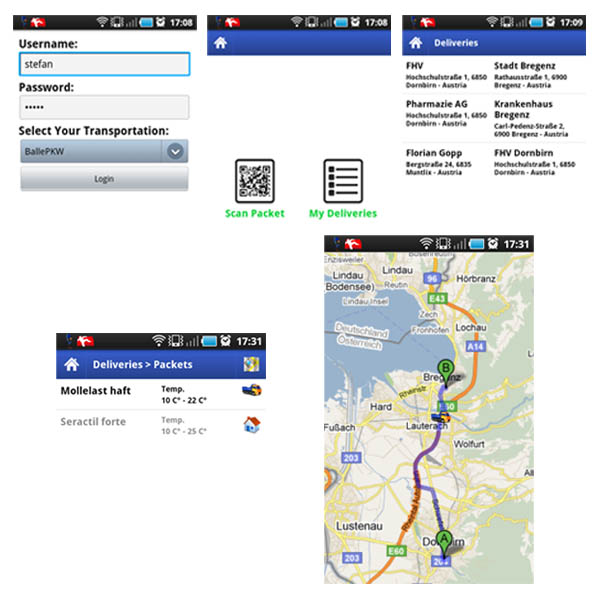
\includegraphics[width=140mm]{files/AndroidApp.jpg}

\section{Kommerzielle Temperatursensoren}
	\paragraph{Hygrosens TLOG20-BLUE}
		Das ist \textit{NICHT} unsere Lösung.
		\url{http://shop.hygrosens.com/Messsysteme-acma/
			Messsysteme-fuer-Temperatur/Temperaturmesssysteme/
			Temperaturmesssysteme-BLUETOOTH/
			BLUETOOTH-Temperaturmesssystem-20-Kanaele.html}
			{hygrosens.com/TLOG20-BLUE, Zugriff am 16.04.2011}
	\par
	
	\paragraph{Ampedrf BT11}
		Das ist \textit{NICHT} unsere Lösung.
		\url{http://www.ampedrf.com/modules.htm}
		{BT11 Class1, Zugriff am 16.04.2011}
		\url{http://www.ampedrf.com/datasheets/BT11_Datasheet.pdf}
		{BT11 Datasheet}
	\par 

	\paragraph{\$149 Programmable Universal Key Fob Sensor}
		Wir haben uns für das BlueRadios BR-FOB-SEN-LE4.0 Device  entschieden, weil es
		eine komplette und etablierte Lösung für Temperatur, Beschleunigungs- und
		Licht-Messung ist.
		\url{http://www.blueradios.com/BR-FOB-SEN-LE4.0-S2A.pdf}
		{Blueradios BR-FOB-SEN-LE4, Zugriff am 16.04.2011}
		
		\url{http://www.blueradios.com/hardware_sensors.htm}
		{Blueradios BR-FOB-SEN-LE4}
	\par
	
\end{appendix}



% ende des hauptteils
\fancyhead[R]{} % Keine Kopfzeile mehr oben auf jeder Seite

\end{document}
